\section{Trames LoRaMAC}\label{sec:archi-loramac-frame}
\renewcommand{\rightmark}{Trames LoRaMac}

    Le protocole MAC mis en place pour les communications LoRa utilise un seul format de trames illustré à la figure~\ref{fig:archi-frame}.
    \begin{figure}[H]
        \centering
        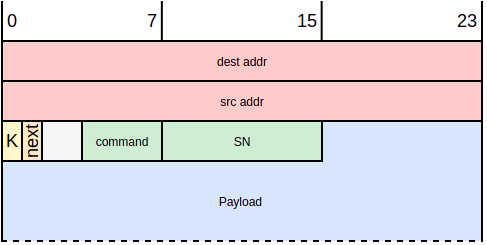
\includegraphics[scale=0.5]{res/pictures/loramac-frame.drawio.png}
        \caption{Format de trame LoRaMAC.}
        \label{fig:archi-frame}
    \end{figure}
    Les trames LoRaMAC sont composées des champs suivants:
    \begin{itemize}
        \item \textbf{dest\_addr}: l'adresse de destination (24 bits)
        \item \textbf{src\_addr}: l'adresse source (24 bits)
        \item \textbf{K}: un flag  qui indique si la trame nécessite un acquittement (1 bit)
        \item \textbf{next}: un flag qui indique si une autre trame suit (1 bit)
        \item \textbf{reserved}: 2 bits réservés pour évolution future
        \item \textbf{command}: la commande MAC (4 bits).\\
        Les 5 commandes disponibles ainsi que leurs valeurs sont reprises dans la table~\ref{tb:archi-loramac-command}. Il est possible d'ajouter 10 commandes supplémentaires pour des usages futurs.
        \item \textbf{SN}: le numéro de séquence de la trame (8 bits)
        \item \textbf{Payload}: la payload ayant une taille maximale de 247 octets. Cette limitation provient de la radio LoRa utilisée, le RN2483, qui limite les transmissions à 255 octets, valeur de laquelle est soustrait les 8 octets des champs précédents.
        \begin{table}[H]
            \centering
            \makebox[\textwidth]{%
            \begin{tabular}{|c|c|c|c|}
                \hline
                Valeur & Commande & description & payload\\ \hline
                0 & JOIN & requête pour rejoindre le réseau & $\times$ \\ \hline
                1 & JOIN\_RESPONSE & réponse à la commande JOIN & préfixe du sous réseau\\ \hline
                2 & DATA & transport de données & données\\ \hline
                3 & ACK & acquittement & $\times$\\ \hline
                4 & QUERY & demande de trafic descendant & $\times$\\ \hline
            \end{tabular}
            }
            \caption{Description des commandes LoRaMAC.}
            \label{tb:archi-loramac-command}
        \end{table}
    \end{itemize}
